\documentclass[conference]{IEEEtran}

\usepackage[T1]{fontenc}
\usepackage[utf8]{inputenc}
\usepackage{amsmath,amssymb}
\usepackage{array}
\usepackage{booktabs}
\usepackage{cite}
\usepackage{graphicx}
\usepackage{microtype}
\usepackage{placeins}
\usepackage{url}
\usepackage[table]{xcolor}

\graphicspath{{figures/}}
\setlength{\textfloatsep}{6pt plus 1pt minus 2pt}
\setlength{\dbltextfloatsep}{7pt plus 1pt minus 2pt}
\setlength{\floatsep}{5pt plus 1pt minus 2pt}
\setlength{\intextsep}{5pt plus 1pt minus 2pt}
\setlength{\abovecaptionskip}{3pt}
\setlength{\belowcaptionskip}{2pt}

\title{Physics-Informed Hierarchical Tree Ensembles for\\
Sparse-PMU Event Detection and Localization}

\author{
\IEEEauthorblockN{Jorge Luis Mayorga Taborda and Yessica Africano Rodriguez}
\IEEEauthorblockA{Universidad de los Andes, Bogot\'a, Colombia}
}

\begin{document}
\maketitle

\begin{abstract}
Event localization is indirect when PMU coverage is sparse: only eight of the 39 buses are instrumented in the SGSMA 2026 task. Our system describes local transients and their propagation across PMUs, then routes each event to a BUS, LINE, or PMU localizer. We compare flat, typed, and typed+topology tree ensembles on 690 IEEE 39-bus simulations. All three use past-only 3-s windows, whole-scenario splits, validation-selected thresholds, and 360 trees. Flat obtains 0.977 detection F1 and 0.535 row-level physical Top-1, compared with 0.965 and 0.496 for typed. Typed reduces serialized model size from 98.3 to 28.1 MB and halves model-only prediction time. Its scenario-level localization estimate is 0.614, versus 0.590 for flat, although the paired interval includes zero. Adding effective electrical distance in the typed+topology ranker gives no localization gain under the evaluated configuration. Missing-only events remain unresolved. Because every target appears during training, these results measure new trajectories at known assets, not localization at unseen targets.
\end{abstract}

\begin{IEEEkeywords}
event localization, hierarchical classification, non-anticipation, phasor measurement units, physics-informed machine learning, synchrophasors.
\end{IEEEkeywords}

\section{Introduction}
The SGSMA 2026 task asks for three outputs at every timestamp: normal or abnormal status, an event label from 0 to 8, and a location \cite{sgsmaGuide2026,sgsmaPolicy2026}. Yet only eight buses are observed in the IEEE 39-bus system. Voltage, angle, current, frequency, and rate-of-change-of-frequency describe what happens at an instrumented bus \cite{phadke2008,ieee2018}; they do not identify an unobserved origin on their own. Localization therefore depends on how the disturbance appears across PMUs and on the electrical paths between the observed and candidate assets.

Our hackathon system was built around that distinction. Local-reference departures describe the size and persistence of a transient at one PMU. Rolling summaries and adaptive prediction errors describe its evolution, while cross-PMU contrasts capture relative severity and timing. ExtraTrees models first reconcile physical-event and measurement-integrity evidence. The predicted event then selects the appropriate origin space: BUS, LINE, or PMU. A parallel network path derives effective electrical distance from $Y_{\mathrm{bus}}$ and $Z_{\mathrm{bus}}$ (Fig.~\ref{fig:system}).

The task requires a label at each timestamp, whereas the archived executable predicts once from a complete 30-s segment and copies the result to every row. We therefore retain the submitted representation and hierarchy but evaluate temporal behavior with a past-only implementation. A second evaluation check concerns the candidate universe: a localizer cannot recover an admissible asset that is absent from its fitted classes. Precision, alarm episodes, and delay measure temporal behavior; candidate coverage, Top-$k$ recovery, and electrical-distance error measure spatial behavior.

We reconstructed the feature map, routing logic, and candidate spaces from the executable, then built a past-only benchmark with whole-scenario splits. Flat, typed, and typed+topology models share trajectories, validation rules, seeds, and a 360-tree budget. The experiments ask whether typed heads offer a useful accuracy--size trade-off and whether a candidate ranker supplied with electrical distance improves localization. Because the ranker also changes the localizer architecture and training representation, the second comparison does not isolate electrical distance.

\section{Related Work}
PMU event identification has been approached through statistical and physics-based variables, modal analysis, and learned interactions among measurements \cite{pandey2020,taghipour2023,yuan2023gnn}. Missing or corrupted records need a distinct treatment because their signatures may resemble a physical transient \cite{yuan2021,liu2023}.

Localization adds a spatial inference problem. Prior methods infer faulted lines jointly \cite{li2019}, learn patterns under sparse PMU placement \cite{yildiz2024}, or represent the grid through graphs and multiple measurement sources \cite{ahmed2024,ganjkhani2024}. Network knowledge has also been introduced directly into transmission-grid models \cite{li2024knowledge}, through connectivity, impedance-derived distance, candidate variables, or physical constraints. Here effective distance serves two roles. The submitted representation can use it to weight cross-PMU contrasts, although the archived inference call left those weights at one. The typed+topology variant supplies distance explicitly to a candidate ranker.

\section{Physics-Informed Hierarchical Diagnosis}
\subsection{Sparse-PMU evidence representation}
Figure~\ref{fig:system} summarizes the complete diagnostic path. Eight synchronized PMUs observe buses $\{2,5,6,10,19,22,29,39\}$. Within each PMU, the representation measures departure from normal operation and tracks that departure through pre-event, early, middle, and late intervals. Across PMUs, it compares severity, timing, correlation, and lag. The submitted 30-s extractor expands these two views into the five feature blocks in Table~\ref{tab:featuremap}.

\begin{table}[!t]
\centering
\caption{Feature map reconstructed from the archived schema.}
\label{tab:featuremap}
\scriptsize
\setlength{\tabcolsep}{3pt}
\begin{tabular}{@{}lrl@{}}
\toprule
\textbf{Block} & \textbf{Count} & \textbf{Recorded evidence} \\
\midrule
Base & 39,716 & segments, quality, power proxies \\
Metadata & 28 & availability, NaN, and timestamp-gap fields \\
Rolling & 3,360 & level, spread, slope, energy, peak time \\
Residual/innovation & 1,344 & RLS and Kalman prediction errors \\
Spatial-temporal & 714 & PMU-pair severity and timing \\
\midrule
Total & 45,162 & one vector per 30-s segment \\
\bottomrule
\end{tabular}
\end{table}

Network information is derived from the branch admittance model. Effective distance and the corresponding pair weight are
\begin{equation}
\begin{aligned}
Z_{\mathrm{bus}}&=Y_{\mathrm{bus}}^{+},\\
d_{ab}^{\mathrm{eff}}&=|Z_{aa}+Z_{bb}-Z_{ab}-Z_{ba}|,\\
\omega_{ab}&=(d_{ab}^{\mathrm{eff}}+\epsilon)^{-1}.
\end{aligned}
\label{eq:distance}
\end{equation}
Small $d_{ab}^{\mathrm{eff}}$ indicates that buses $a$ and $b$ are electrically close, even when they are far apart in the one-line drawing. The inverse weight gives greater influence to such pairs. Signal departures are measured relative to the first 3 s of each PMU channel. For signal $s$ at PMU $p$,
\begin{equation}
\begin{aligned}
b_{p,s}&=\mathop{\mathrm{med}}_{\tau\in S_0}x_{p,s}(\tau),\\
\sigma^{\mathrm{rob}}_{p,s}&=1.4826\,\mathop{\mathrm{med}}_{\tau\in S_0}|x_{p,s}(\tau)-b_{p,s}|,\\
z_{p,s}(t)&=|x_{p,s}(t)-b_{p,s}|/(\sigma^{\mathrm{rob}}_{p,s}+\epsilon).
\end{aligned}
\label{eq:baseline}
\end{equation}
The median and median absolute deviation reduce sensitivity to isolated spikes in the reference interval. Peak $z_{p,s}$ measures excursion size; persistence records how long the excursion remains large. Rolling windows of 5, 15, 30, 60, and 120 samples then describe transients at several time scales. Two predictors measure departures from recent behavior, and a pairwise term compares PMUs:
\begin{equation}
\begin{aligned}
r_t^{(\lambda)}&=\left|y_t-\boldsymbol{\phi}_t^\top
\boldsymbol{\theta}_{t-1}^{(\lambda)}\right|, &
\nu_t&=\left|y_t-\hat{x}_{t-1}\right|,\\
g_{ab}&=\omega_{ab}\max_t|y_{a,t}-y_{b,t}|.
\end{aligned}
\label{eq:dynamic}
\end{equation}
The RLS residual $r_t^{(\lambda)}$ uses $\lambda\in\{0.92,0.985\}$ and $\boldsymbol{\phi}_t=[1,t-t_0]^\top$; a constant-level tracker runs alongside it. A scalar level filter sets $Q=(0.005s)^2$ and $R=(0.08s)^2$ from channel scale $s$, producing innovation $\nu_t$. The archive retains the mean, 95th percentile, late-to-pre shift, and peak time of these sequences. Spread, correlation, lag, and peak-time difference supply the cross-PMU view. Although the extractor supports $d_{ab}^{\mathrm{eff}}$, the submitted call did not pass it, so $g_{ab}$ used unit pair weights.

\subsection{Hierarchical event and typed origin inference}

The hierarchy separates two questions that have different location spaces: whether the signal indicates a physical event, and whether a PMU record is missing or corrupted. One forest estimates physical classes $\{0,1,2,3,4,8\}$; two integrity forests check missing composition (events 5 and 6) and isolated bad data (event 7). Routing rules combine these scores. Fault, generation, load, and mixed events use BUS candidates; line outages use LINE candidates; missing and bad-data events use PMU candidates. Event 6 follows its physical component. If $C_\tau$ is the candidate set for route $\tau$, then
\begin{equation}
\tau=r(\hat e,\hat e_{\mathrm{phys}}),\qquad
\hat\ell=\arg\max_{\ell\in C_\tau}p_{\mathrm{ET},\tau}(\ell\mid\mathbf{x}).
\label{eq:localizer}
\end{equation}
The submitted bundle contains a 750-tree physical forest, two 650-tree integrity forests, and eight 180-tree localizers. Typed routing keeps measurement failures out of the BUS and LINE candidate spaces and avoids asking one classifier to compare incompatible asset types.

\subsection{Prediction contract and candidate ontology}
For timestamp-level inference, let $X_{\leq t}$ contain the aligned samples available by time $t$. We evaluate predictions of the form
\begin{equation}
(\hat e_t,\hat p_t,\hat q_t)=f\!\left(\Phi(X_{\leq t})\right),
\label{eq:nonanticipation}
\end{equation}
Here $\hat e_t\in\{0,\ldots,8\}$, while $\hat p_t$ and $\hat q_t$ are physical and integrity targets; either target may be empty. The feature map $\Phi$ is \emph{temporally non-anticipative} if changing samples after $t$ leaves the prediction at $t$ unchanged. This interpretation follows the policy's requirement for a label at every timestamp and the guide's use of streaming delay and false alarms \cite{sgsmaGuide2026,sgsmaPolicy2026}. The recommended window length is treated as guidance for the online pipeline, not as a restriction on separate offline analysis.

Candidate coverage is evaluated against the supplied network rather than the labels seen during training. Its branch file contains 34 transmission lines and 12 transformers after taps and phase shifts are accounted for. The task defines 39 fault buses, 34 line candidates, 10 generator reporting buses, 18 load buses, and eight integrity sites. For fitted labels $\mathcal L_e$ and valid candidates $\mathcal C_e$, we report $\operatorname{cov}(e)=|\mathcal L_e\cap\mathcal C_e|/|\mathcal C_e|$ and $\operatorname{inv}(e)=|\mathcal L_e\setminus\mathcal C_e|$. Integrity sites are reported as bus labels, following the guide; the PMU identifier is not assumed to equal its bus number.

\subsection{Submitted system and benchmark alignment}
We read the promoted localizer bundle directly from the submitted ZIP archive (SHA-256 prefix e0bfc17e4c5e). After normalizing reversible naming differences, we compared every fitted class with the candidate sets above. The resulting inventory records valid, missing, and out-of-ontology labels and can be reproduced from the evidence JSON.

Two implementation details prevent a direct timestamp-level interpretation of the original scores. First, the executable makes one prediction from a complete 30-s segment and copies it to every row, so an early-row prediction can depend on later samples. Second, its line localizer uses a different branch universe from the task. Of 34 fitted labels, 24 are valid transmission lines and 10 are step-up transformers, while 10 admissible lines are absent; hence $\operatorname{cov}(2)=24/34$ and $\operatorname{inv}(2)=10$. The other label differences are reversible. Device buses 30--39 map one-to-one to the 10 high-side generator reporting buses. The load localizer contains all 18 valid buses plus BUS31, which lies outside the load candidate set.

\begin{figure*}[!t]
\centering
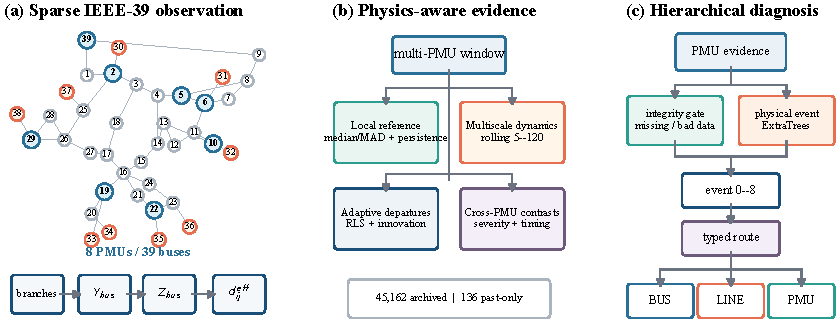
\includegraphics[width=\textwidth]{fig1_system_reconstruction.pdf}
\caption{Physics-informed hierarchical diagnosis. (a) Eight PMUs observe the IEEE 39-bus system; the branch model defines $Y_{\mathrm{bus}}$, $Z_{\mathrm{bus}}$, and effective distance. (b) Local-reference, multiscale, adaptive-residual, and cross-PMU views describe each segment. (c) Integrity and physical evidence are reconciled before localization over BUS, LINE, or PMU candidates. Prototype pair weights defaulted to one; typed+topology receives effective distance explicitly.}
\label{fig:system}
\end{figure*}

\begin{table*}[!t]
\centering
\caption{Transition from the presented design to the controlled evaluation. Counts come from the serialized model and supplied network files.}
\label{tab:runtime}
\renewcommand{\arraystretch}{1.05}
\scriptsize
\begin{tabular}{@{}p{0.15\textwidth}p{0.25\textwidth}p{0.27\textwidth}p{0.25\textwidth}@{}}
\toprule
\textbf{Item} & \textbf{Presented design} & \textbf{Prototype realization} & \textbf{Controlled evaluation} \\
\midrule
Decision time & One label per timestamp using available samples & Complete 30-s segment; one label copied to all rows & Trailing 3-s window; one prediction at every row \\
Representation & Past-only variables with documented network inputs & 45,162 variables; spatial-temporal pair weights default to 1.0 & 136 trailing-window variables; ranker receives electrical distance \\
Line outage & 34 transmission-line labels & 24 valid lines, 10 valid lines absent, 10 transformer labels & All and only the 34 lines occur in every split \\
Generation & 10 high-side reporting buses & 10 low-side device-bus labels & Deterministic 10-to-10 report-bus map \\
Load & 18 nonzero-load buses in the supplied RAW case & All 18 plus BUS31 & BUS31 excluded from the candidate universe \\
Integrity & Eight instrumented bus locations & Labels use a \texttt{PMU} prefix with a bus suffix & Canonical \texttt{BUS} labels; official PMU-to-bus map retained \\
Evidence & Scenario-level split; labeled test for performance & Inspected development and selection sets; hidden streams unlabeled & Whole-scenario train/validation/test partition \\
\bottomrule
\end{tabular}
\end{table*}

The development report gives 0.9693 detection accuracy, 0.9598 event macro-F1, and 1011/1186 exact locations on the inspected simulation split. Its selected representation reaches 0.8524 localization Top-1; a smaller variant reaches 0.8558. The same process compared 16 representations on RAW0001 and selected one that recovered 8/12 locations. Because those data guided representation choice, the figures are development-set rather than held-out estimates. The unlabeled competition streams confirm executable inference but cannot support a performance estimate. Inference and the schema/class checks are reproducible from the archive; training is not, because the original corpus and feature tables were not retained.

\section{Non-Anticipative Evaluation}
\subsection{Scenario design and split}
The benchmark contains 690 five-second ANDES simulations of the IEEE 39-bus case \cite{athay1979,cui2021andes}. Every event begins at 2 s. Faults last 0.2 s; line outages and operating changes persist; missing or corrupted measurements last 0.7 s. We estimate scale, noise, and sampling rate from the normal rows of RAW0001, then use those values only to calibrate the simulations. RAW labels are not used for fitting or threshold selection. Five replicas of each target vary event severity, operating scale, and simulator seed.

The 138 target keys cover one normal case, 39 fault buses, 34 lines, 10 generator buses, 18 load buses, eight missing-data sites, 10 generation-plus-missing cases, eight bad-data sites, and 10 mixed cases. Event 8 combines generator and load changes with one corrupted PMU. For every key, three replicas are assigned to training, one to validation, and one to test, producing 414/138/138 whole-scenario partitions. Test trajectories are excluded from fitting and threshold selection. Because each target appears in every partition, this is a supervised, target-covered experiment: it tests new trajectories at known assets.

\begin{figure*}[!t]
\centering
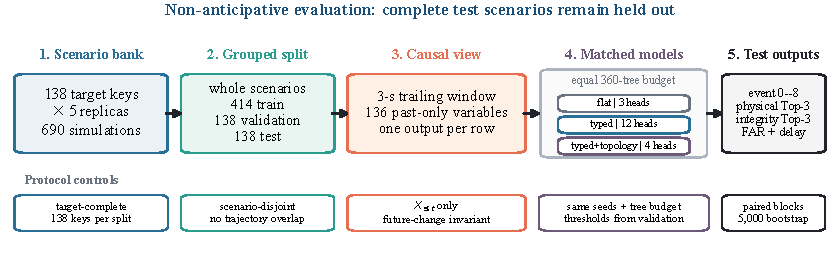
\includegraphics[width=\textwidth]{fig2_causal_protocol.pdf}
\caption{Non-anticipative evaluation protocol. Target-covered splits separate complete trajectories. All baselines use the same past-only PMU variables, data, model seeds, and tree budget; the ranker adds static candidate-distance variables.}
\label{fig:protocol}
\end{figure*}

\subsection{Past-only features and matched baselines}
At timestamp $t$, the causal extractor reads no more than the preceding 3 s; during startup, it uses the history available so far. For voltage magnitude, unwrapped angle, and frequency, each PMU contributes the current value, departure from its first available value, mean, standard deviation, and slope. Missing fraction and disturbance score bring the total to 17 features per PMU, or 136 overall. A unit test changes samples after $t$ and verifies that features at and before $t$ remain unchanged.

All variants use ExtraTrees with depth 14, at least two samples per leaf, square-root feature subsampling, and \texttt{class\_weight=balanced\_subsample} \cite{geurts2006,pedregosa2011}. Since bootstrap is disabled, scikit-learn 1.7.2 applies global balanced sample weights. The \emph{flat} variant allocates 120 trees to each of three heads: event, physical location, and integrity location. The \emph{typed} variant divides the event stage into binary detection and abnormal-event classification, then assigns separate location heads by event type. Its tree counts still sum to 360. For both variants, validation chooses the abnormal threshold from the same 33-value grid. The \emph{typed+topology} variant retains the typed event stage but replaces the location heads with two candidate rankers. A ranker row combines PMU disturbance scores with candidate type, electrical distances to the eight PMUs, distance summaries, and score interactions weighted by $\exp(-d)$. It also uses 360 trees.

\subsection{Metrics}
Detection is evaluated by abnormal precision, recall, F1, false-positive fraction, alarm episodes per normal-labeled minute, scenario detection, and delay. Event scores use the fixed labels 0--8. For physical and integrity locations, we report row-level Top-1/Top-3, coverage, and electrical-distance error. Scenario Top-1 is the modal prediction over target-active rows. Empty outputs vote as \texttt{NONE}; ties are resolved by whichever candidate first reached Top-1. Prediction time excludes feature computation. We ran the models with \texttt{n\_jobs=-1} on an Intel Core Ultra 9 185H (16 physical/22 logical cores), 31.5 GB RAM, and Windows 11. Each seed was timed once without warm-up. Confidence intervals come from 5000 paired bootstrap replicates that resample scenarios within event type and keep model seeds paired.

\subsection{Reproducibility controls}
Each run stores scenario seeds, split manifests, input hashes, and all test predictions. Before fitting, checks reject partition overlap, missing targets, invalid routed labels, non-finite trajectories, and simulations shorter than 5 s; all 690 scenarios pass. The non-anticipation test described above checks the feature code directly. The only validation-selected quantities are abnormal thresholds, chosen from 33 fixed values between 0.1 and 0.9.

\section{Results}
Validation selects an abnormal threshold of 0.75 for flat and 0.45 for typed in all three seeds. At those thresholds, flat reaches $0.995\pm0.0004$ precision, $0.959\pm0.001$ recall, and $0.977\pm0.001$ F1. Typed reaches $0.981\pm0.001$, $0.951\pm0.002$, and $0.965\pm0.002$, respectively. The paired interval for typed minus flat F1 is $[-0.0207,-0.0045]$. Flat also has a lower false-positive fraction (0.0029 versus 0.0120). Its alarm rate is 3.22 episodes per normal-labeled minute, compared with 4.01 for typed, although the paired FAR interval $[-1.21,2.94]$ includes zero. Of 137 abnormal scenarios, flat detects 130 with $0.0189\pm0.0008$ s mean delay; typed detects 129 with $0.0287\pm0.0035$ s delay. Table~\ref{tab:results} and Fig.~\ref{fig:results} give the remaining aggregate results.

\begin{table*}[!t]
\centering
\caption{Non-anticipative test results across three seeds, with mean $\pm$ sample standard deviation where shown. S@1 is modal physical Top-1 per scenario. FAR is episodes per normal-labeled minute; runtime excludes feature computation.}
\label{tab:results}
\renewcommand{\arraystretch}{1.08}
\scriptsize
\setlength{\tabcolsep}{3.3pt}
\begin{tabular}{@{}lcccccccccc@{}}
\toprule
\textbf{Method} & \textbf{Det. P} & \textbf{Det. R} & \textbf{Det. F1} & \textbf{Event M-F1} & \textbf{Phys. S@1} & \textbf{FAR} & \textbf{Phys. @1/@3} & \textbf{Integ. @1/@3} & \textbf{s/min} & \textbf{nodes/ser. MB} \\
\midrule
Flat & $\mathbf{.995\pm.000}$ & $\mathbf{.959\pm.001}$ & $\mathbf{.977\pm.001}$ & $\mathbf{.800\pm.006}$ & $.590\pm.017$ & $\mathbf{3.22\pm.14}$ & $\mathbf{.535/.671}$ & $\mathbf{.888/.888}$ & $.051$ & $282$k/$98.3$ \\
Typed & $.981\pm.001$ & $.951\pm.002$ & $.965\pm.002$ & $.791\pm.011$ & $\mathbf{.614\pm.029}$ & $4.01\pm.40$ & $.496/.646$ & $.870/.874$ & $\mathbf{.025}$ & $176$k/$28.1$ \\
Typed+topology & $.981\pm.001$ & $.951\pm.002$ & $.965\pm.002$ & $.791\pm.011$ & $.581\pm.029$ & $4.01\pm.40$ & $.462/.622$ & $.874/.876$ & $.586$ & $290$k/$25.7$ \\
\bottomrule
\end{tabular}
\end{table*}

\begin{figure*}[!t]
\centering
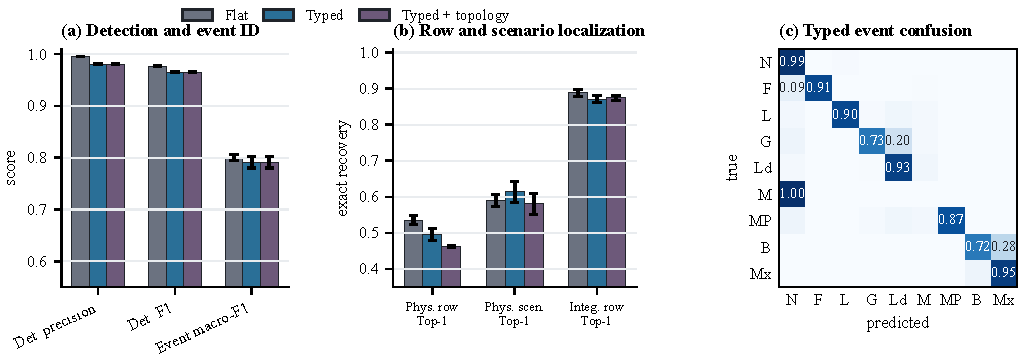
\includegraphics[width=\textwidth]{fig3_causal_results.pdf}
\caption{Test trade-offs after validation threshold selection. Error bars show one sample standard deviation across seeds. Scenario Top-1 uses the modal candidate and counts an empty output as an error. The confusion matrix pools the typed runs. N: normal, F: fault, L: line, G: generation, Ld: load, M: missing, MP: missing plus physical, B: bad data, Mx: mixed.}
\label{fig:results}
\end{figure*}

\begin{figure*}[!t]
\centering
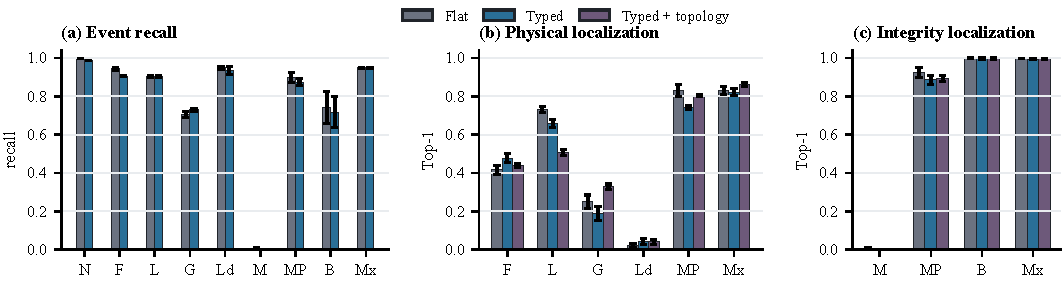
\includegraphics[width=\textwidth]{fig4_per_event_diagnostics.pdf}
\caption{Per-event test diagnostics, mean with one sample standard deviation across seeds. Event abbreviations follow Fig.~\ref{fig:results}. Event recall is identical for typed and typed+topology because they share the event stage. Location scores count an empty or misrouted output as incorrect.}
\label{fig:per-event}
\end{figure*}

Event macro-F1 is 0.800 for flat and 0.791 for typed; weighted-F1 is 0.949 and 0.941. Most of the remaining classification error is concentrated in two classes. Typed assigns every missing-only test row to normal, and flat recalls only $0.006\pm0.006$ of that class. Generation-change recall is 0.705 for flat and 0.729 for typed. The deterministic absence pattern in missing-only events suggests that a presence gate should be evaluated separately from the learned event classifier.

Localization depends on the unit of analysis. By row, physical Top-1 is $0.535\pm0.012$ for flat and $0.496\pm0.017$ for typed, with a typed-minus-flat interval of $[-0.0772,-0.0029]$. After predictions are pooled within each scenario, typed has the higher point estimate: $0.614\pm0.029$ versus $0.590\pm0.017$. The corresponding interval, $[-0.0551,0.1019]$, includes zero. Physical coverage is 0.949 for flat and 0.943 for typed; integrity Top-1 is 0.888 and 0.870.

Typed+topology reaches 0.462 physical Top-1 by row and 0.581 by scenario. Relative to typed, the intervals are $[-0.0734,0.0047]$ and $[-0.1129,0.0441]$. Prediction time rises from 0.025 to 0.586 s per input minute. Because candidate pooling, the number of training rows, and the localizer heads change together with the distance variables, this comparison cannot assign the difference to electrical distance alone.

The per-event results in Fig.~\ref{fig:per-event} show where the aggregate loss occurs. Relative to typed, typed+topology improves generation-change Top-1 from 0.188 to 0.328, missing-plus-physical from 0.741 to 0.804, and mixed events from 0.822 to 0.860. For line outages, however, Top-1 falls from 0.658 to 0.507. That class accounts for 3128 of the 7915 physical test rows. Load localization remains below 0.05 for every method. Integrity sites for bad-data and mixed events are recovered in nearly every correctly routed row; missing-only rows rarely reach an integrity localizer because the event stage labels them normal.

\section{Discussion}
The flat and typed variants favor different costs. Flat has higher detection F1 and row-level physical Top-1. Typed reduces serialized size by 71\% and halves model-only prediction time. Pooling rows within a scenario reverses the localization point estimates, but the paired interval includes zero. The evidence therefore supports the storage and timing advantage of typed heads, not a scenario-level accuracy advantage.

The role of network information is less settled. Several variables in the submitted representation have a physical interpretation: local departures, adaptive residuals, power proxies, and cross-PMU timing. Explicit network structure enters the evaluated models only through effective distance in typed+topology. That variant also changes the candidate representation and the construction of training rows. A controlled distance ablation would keep those choices fixed and withhold targets, rather than trajectories alone, from fitting. Under the present target-covered split, a class localizer can learn an asset-specific signature without learning how to rank an unseen asset.

Missing-only events expose a different failure. Their absence pattern is deterministic, yet the event stage sends almost every row to normal. A simple presence gate is a plausible remedy, although its effect on false alarms and delay remains to be measured. More generally, the reported rates come from one simulated network, one PMU placement, known targets, and 7.15 min of normal-labeled data, mostly before event onset. RAW0001 calibrates the simulations but does not provide field validation. Longer normal records, repeated splits, broader event schedules, learning curves, and a temporal baseline would be needed to assess transfer beyond this setting.

\FloatBarrier
\section{Conclusion}
On the target-covered IEEE 39-bus benchmark, flat heads give higher detection and row-level localization scores, while typed heads use less serialized model storage and prediction time. Scenario aggregation yields no clear localization difference. Supplying effective electrical distance through a candidate ranker does not improve the reported scores under the current comparison, which also changes the localizer and its training representation. A fixed-architecture, leave-target-out ablation is the next test of the distance contribution.

\bibliographystyle{IEEEtran}
\IEEEtriggeratref{4}
\bibliography{references}

\end{document}
